Ein RC-Schwingkreis besteht in der Regel aus einem Kondensator mit der
Kapazität $C$ und einer Spule, die eine Induktivität $L$ liefert.
Diese beiden Bauteile dienen hier als Energiespeicher.
In einem idealen Schwingkreis wird eine einmal eingespeicherte Energie
immer zwischen beiden genannten Elementen ausgetauscht.
Dieser Austausch kommt durch die Entladung des Kondensators zustande, bei welcher
in der Spule ein Magnetfeld aufgebaut wird. Wird dieses Magnetfeld abgebaut,
lädt sich der Kondensator auf und der Vorgang beginnt von neuem.
Wird ein gedämpfter, also ein realer Schwingkreis, betrachtet, ist neben der
Spule und dem Kondensator noch ein ohmscher Widerstand $R$ vorhanden.
Über diesen wird die Energie in Wärme umgewandelt und somit aus dem
Schwingkreis entfernt. $R$ ist demnach ein Dämpfungsfaktor.
Der schematische Aufbau eines $RCL$-Schwingkreises ist in Abbildung \ref{fig:rcl}
zu sehen.
\begin{figure}[H]
  \centering
  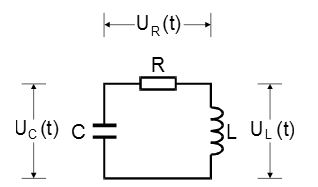
\includegraphics{Bilder/RCL.JPG}
  \caption{Schematischer Aufbau eines $RCL$-Kreises\,\cite{354}}
  \label{fig:rcl}
\end{figure}
Die Werte von $U_\su{R}, U_\su{C}$ und $U_\su{L}$ bezeichnen hierbei die Spannung
die über dem jeweiligen Bauteil abfällt. Gemäß des 2. Kirchhoffschen Gesetzes
gilt:
\begin{equation}
  U_\su{R}(t) + U_\su{C}(t) + U_\su{L}(t) = 0.
  \label{eqn:kirch}
\end{equation}
Um eine Differentialgleichung der 2. Ordnung zu erhalten, wird die Spannung
durch den Strom $I$ ausgedrückt. Somit erhält man:
\begin{align*}
  U_\su{R}(t) &= RI(t) \\
  U_\su{C}(t) &= \frac{Q(t)}{C} \qquad \text{mit} \qquad I = Q \\
  U_\su{L}(t) &= LI ,
\end{align*}
was zu der Differentialgleichung
\begin{equation}
  I(t) + \frac{R}{L}I(t) + \frac{1}{LC} I(t) = 0 .
\end{equation}
Mit dem entsprechendem Ansatz ergibt sich für die Gleichung die Lösung
\begin{equation}
  I(t)=\su{e}^{-2\pi\mu t}(A_1\su{e}^{i2\pi\nu t} + A_2\su{e}^{-2i\pi\nu t}).
  \label{eqn:dgl}
\end{equation}
Die Parameter $\mu$ und $\nu$ sind dabei definiert als:
\begin{align}
  \mu &\coloneqq\frac{R}{4\pi L}\label{eqn:reff} \\
  \nu &\coloneqq\frac{1}{2\pi}\sqrt{\frac{1}{LC}-\frac{R^2}{4\L^2}}
\end{align}
Für $\nu$ muss aufgrund der Wurzel eine Fallunterscheidung gemacht werden, da
$\nu$ sowohl reell, als auch rein imaginär sein kann.
Für den reellen Fall muss
\begin{equation*}
  \frac{1}{LC} > \frac{R^2}{4L^2}
\end{equation*}
gelten. Unter diesen Voraussetzungen lässt sich Formel \eqref{eqn:dgl} mit der
Eulerschen Formel zu
\begin{equation}
  I(t)=A_\su{0}\su{e}^{-2\pi\mu t}\cos(2\pi\nu t+\mu)
  \label{eqn:einh}
\end{equation}
umschreiben. Hier entsteht eine gedämpfte Schwingung, welche bei
$t\rightarrow\infty$
gegen Null strebt. Die Abklingdauer dieser Schwingung wird dann durch
\begin{equation}
  T_\su{ex}\coloneqq\frac{1}{2\pi\mu} \label{eqn:tex}
\end{equation}
definiert.

Für den Fall, dass $\nu$ imaginär ist, also
\begin{equation*}
  \frac{1}{LC} < \frac{R^2}{4L^2} ,
\end{equation*}
lässt sich Formel \eqref{eqn:dgl} zu
\begin{equation}
  I(t)\propto\su{e}^{-(2\pi\mu -\su{i}2\pi\nu)t}
\end{equation}
umschreiben.
Da sich i und $\nu$ zu einem insgesamt reellen Exponenten verrechnen lassen, fällt
die Amplitude des Stroms exponentiell ab. Die Amplitude hat dabei, je nach
Anfangsbedingungen, einen oder keinen Extremwert. Am schnellsten fällt die
Amplitude, wenn der Spezialfall
\begin{equation}
  \frac{1}{LC} = \frac{R^2}{4L^2}
  \label{eqn:r_ap}
\end{equation}
eintritt. Dieser Fall wird aperiodischer Grenzfall genannt und ist in der
Abbildung \ref{fig:agf} als gestrichelte Linie dargestellt.
\begin{figure}[h]
  \centering
  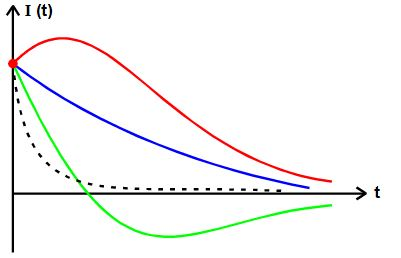
\includegraphics{Bilder/aperiod.JPG}
  \caption{Zeitverlauf des Stroms mit aperiodischer Dämpfung\,\cite{354}}
  \label{fig:agf}
\end{figure}
\\
Abbildung \ref{fig:angeregt} zeigt einen $RCL$-Schwingkreis, welcher von
außen angeregt wird. Die Anregung erfolgt hier durch eine Wechselspannung.
\begin{figure}[h]
  \centering
  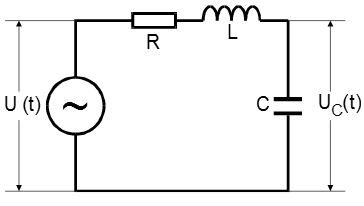
\includegraphics{Bilder/angeregt.JPG}
  \caption{Schaltbild eines angeregten $RCL$-Schwingkreises\,\cite{354}}
  \label{fig:angeregt}
\end{figure}
Nach einer kurzen Einschwingzeit nimmt der Schwingkreis die Frequenz der
Wechselstromquelle an. Die zu Beginn aufgestellte Differentialgleichung aus
Formel \eqref{eqn:dgl} wird nun inhomogen und lautet:
\begin{equation}
  LCU_\su{C}(t) + RCU_\su{c}(t) + U_\su{c}(t) =U_0\su{e}^{\su{i}\omega t}.
  \label{eqn:inh}
\end{equation}
Die Lösung für die Spannung in Abhängigkeit der Zeit berechnet sich dann mit:
\begin{equation}
  U(t)=\frac{U_0(1-LC\omega^2-\su{i}\omega RC)}{(1-LC\omega^2)^2+\omega^2 R^2 C^2}.
\end{equation}
Für die Phasenverschiebung zur Erregerspannung ergibt sich durch den Vergleich
von Imaginär- und Realteil: %Umformulieren um ':' zu vermeiden!!
\begin{equation}
  \varphi(w)=\arctan\biggr(\frac{\su{Im}(U)}{\su{Re}(U)}\biggl)
  =\arctan\biggr(\frac{-\omega RC}{1-LC\omega^2}\biggl)
\end{equation}
Für die Frequenzen $\omega_1$ und $\omega_2$ gilt bei einer Phasenverschiebung
von $\frac{\pi}{4}$ beziehungsweise $\frac{3\pi}{4}$
\begin{equation}
  \omega_\su{1,2}=\pm\frac{R}{2L}+\sqrt{\frac{R^2}{4L^2}+\frac{1}{LC}}.
  \label{eqn:w12}
\end{equation}

Die Spannung kann zusätzlich mit
\begin{equation}
  U_\su{C}(\omega)=\frac{U_0}{\sqrt{(1-LC\omega^2)^2+\omega^2R^rC^2}}
\end{equation}
in Abhängigkeit von der Frequenz $\omega$ angegeben werden.
Hierbei zeigt sich, dass die Spannungsamplitude für sehr hohe Frequenzen gegen
Null strebt, während sie für kleine Frequenzen gegen $U_0$ strebt.
Die Resonanzfrequenz
\begin{equation}
  \omega_\su{res}=\sqrt{\frac{1}{LC}-\frac{R^2}{2L^2}} \label{eqn:wres}
\end{equation}
beschreibt den Zustand, bei dem $U_\su{C}$ einen Maximalwert erreicht der auch
größer als $U_\su{0}$ sein kann.
Von schwacher Dämpfung wird gesprochen, wenn
\begin{equation}
  \frac{R^2}{2L^2} \ll \frac{1}{LC}
\end{equation}
gilt. In diesem Zustand gilt $\omega_\su{res}\approx\omega_0$, wobei $\omega_0$
die Kreisfrequenz der ungedämpften Schwingung ist und den Wert
\begin{equation}
  \omega_0 =\sqrt{\frac{1}{LC}}
\end{equation}
annimmt. Das Maximum der Kondensatorspannung ist dann um den Faktor
\begin{equation}
  q=\frac{1}{\omega_0RC}
  \label{eqn:guete}
\end{equation}
größer als die Erregerspannung. Der Faktor $q$ wird als Güte des Schwingkreises
bezeichnet.

Eine weitere wichtige Größe ist die Breite der Resonanzfrequenz, welche sich mit
\begin{equation}
  \omega_+ - \omega_- \approx \frac{R}{L}
  \label{eqn:breite}
\end{equation}
berechnen lässt.
